\clearpage
\section{Диаграммы работы контроллера}\label{app:uml}
Контроллер читает требования задачи и~выбирает способ вызова (рисунок~\ref{fig:uml-route}). Ветвь с~одним обращением объединяет три действия модели. Для конфигурации с~повторными попытками рисунок~\ref{fig:uml-iteration} показывает, как эта ветвь обрабатывает ответ и~завершает работу.
\begin{figure}[!ht]
\centering
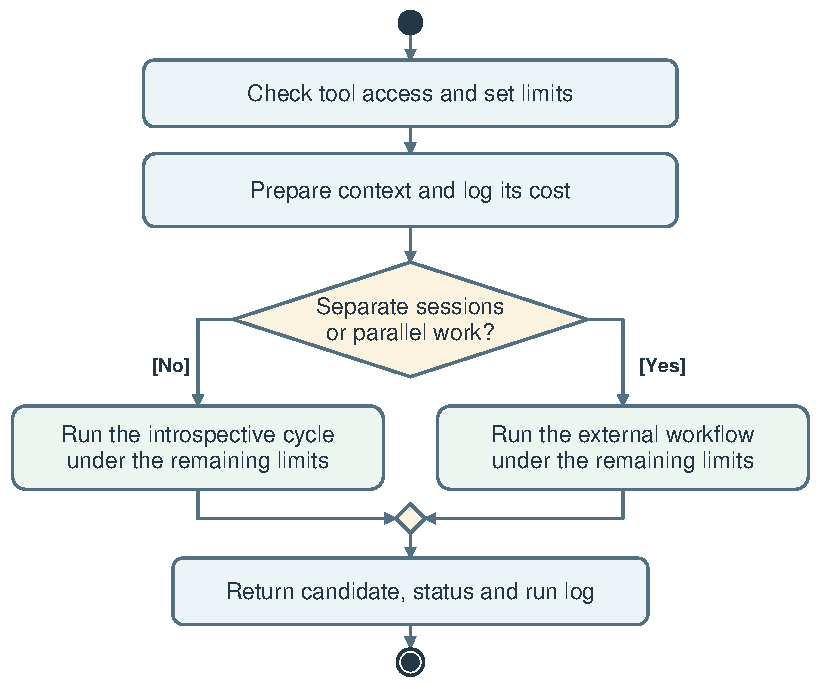
\includegraphics[width=.96\linewidth]{figures/uml-route.pdf}
\caption{Выбор режима и~передача результата. Обе ветви получают оставшиеся лимиты.}\label{fig:uml-route}
\end{figure}
\FloatBarrier
\begin{figure}[!ht]
\centering
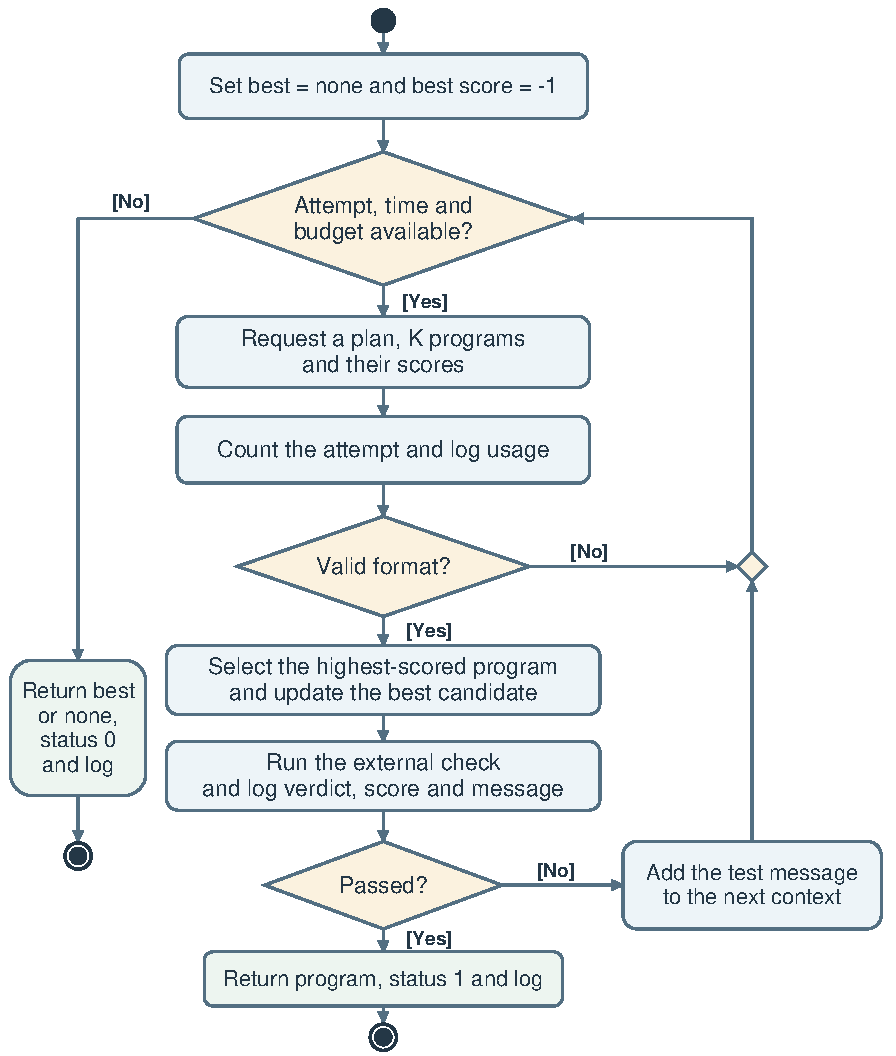
\includegraphics[width=\linewidth,height=.79\textheight,keepaspectratio]{figures/uml-iteration.pdf}
\caption{Интроспективный проход с~проверкой и~ограничением числа попыток. При ошибке формата использованные токены также записываются в~журнал.}\label{fig:uml-iteration}
\end{figure}
\FloatBarrier

\begin{figure}[!ht]
\centering
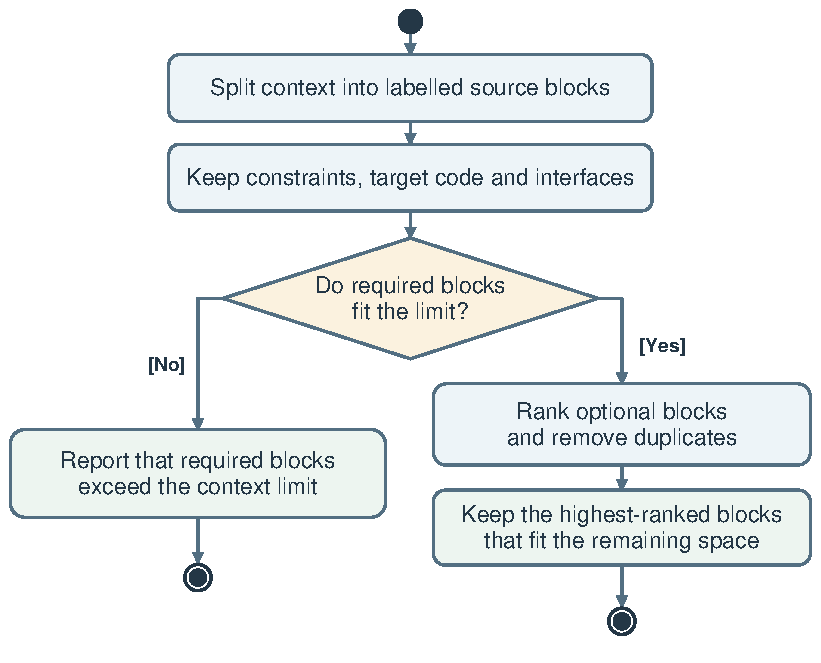
\includegraphics[width=.96\linewidth]{figures/uml-context.pdf}
\caption{Подготовка контекста при включённом сжатии. Если обязательные блоки превышают лимит, контроллер сообщает об~этом до вызова модели.}\label{fig:uml-context}
\end{figure}
\FloatBarrier
\section{Сравнение с~авторской реализацией SCC}\label{subsec:scc}
Self-Collaboration Code Generation, или SCC, сравнивается как более сложная процедура с~взаимодействием ролей и~внутренним исполнением кода. Использован авторский код ревизии \texttt{b471e120}~\cite{scc2024source}. Сохранены классы ролей, инструкции и~логика контроллера. Вызовы адаптированы к~GPT-5.6 Luna через CLI. Число итераций разработчика уменьшено с~четырёх до двух: первоначальный код и~не более одного исправления. Результаты относятся к~этой конфигурации.

Тестировщик SCC создаёт примеры, которые запускаются в~контейнере. Контроллер может остановиться, если выполнение не вызывает исключения. Напечатанные результаты при этом автоматически не сверяются с~ожидаемыми значениями. Поэтому внутреннее завершение SCC ещё не означает успешного решения задачи: окончательная программа отдельно проходит исходные тесты BigCodeBench.

Из 2\,000 назначений каждого метода завершены 1\,600 для SCC, 1\,997 для SR и~1\,998 для SN. Осталось 405 незавершённых запусков: 397 инфраструктурных ошибок и~восемь приостановленных попыток. Большинство ошибок связано с~запуском контейнеров SCC. После контроля среды для SCC доступны 1\,574 оценки, из них 809 успешных. Для SR получено 1\,067 успехов из 1\,964 оценок, для SN --- 1\,064 из 1\,965.

Итоговые тесты и~учёт неуспешных программ остаются такими же, как в~основном сравнении. Однако набор повторов устроен иначе: для задачи заранее выбирались один, два или три повтора, и~часть назначений не завершилась. Поэтому парная оценка SCC использует совпадающие доступные повторы, тогда как в~основной серии требуются все три повтора обоих методов. Сначала разности усредняются внутри задачи, затем задачи получают равные веса. Для SCC минус SR результат равен $-2{,}68$ пункта на 883 задачах с~интервалом $[-4{,}72;-0{,}60]$. Для SCC минус SN получено $-2{,}48$ пункта на 882 задачах с~интервалом $[-4{,}50;-0{,}43]$. Оба значения $p$ после поправки Холма в~отдельном семействе из двух сравнений равны 0,02172.

Большое число пропусков ограничивает этот вывод. Контроль среды прошла 941 из 956 задач этой серии. Если учесть все неизвестные исходы на этих 941 задаче, крайние границы составят $[-12{,}98;+6{,}61]$ пункта относительно SR и~$[-13{,}14;+6{,}43]$ относительно SN. Они допускают оба направления различия. Значит, наблюдаемое преимущество SR и~SN нельзя переносить на всю назначенную выборку SCC.

Для дополнительной проверки сохранены 399 промежуточных программ незавершённых процессов SCC. Из 392 программ на пригодных задачах тесты прошли 196. Это показывает, что инфраструктурный сбой мог прервать процесс уже после появления работающего кода. Но промежуточные программы не подменяют отсутствующий итог контроллера и~не входят в~основную долю успехов SCC.

На полных ресурсных парах отношение средних тарифных оценок SCC/SR равно 3,138 на 896 задачах, а~SCC/SN --- 2,939 на 895. Описательные интервалы составляют $[3{,}07;3{,}21]$ и~$[2{,}87;3{,}01]$. Таким образом, завершённые процедуры SCC с~известными счётчиками требуют больше ресурсов. Неопределённость качества во всей выборке сохраняется из-за пропусков.


\section{Материалы для проверки результатов}\label{app:materials}
Экспериментальная часть сверена с~ревизией \texttt{008b730a} ветки \texttt{FSE-2027} репозитория \href{https://github.com/daniil-novel/article-INoT/tree/008b730a905277079710092ecf3881770eb100fc}{article-INoT}. В~ней доступны архивы ранних серий на 40, 200 и~80 задачах. Данные расширенной серии и~сравнения с~SCC опубликованы в~пакете \path{submission/fse2027/artifact/fse2027-anonymous-analysis-artifact.zip}. Он содержит записи назначений и~сводки: \path{primary/assignment_outcomes.jsonl}, \path{primary/summary.json}, \path{scc/assignment_outcomes.jsonl} и~\path{scc/summary.json}. Этот пакет позволяет пересчитать результаты, но включает не все диалоги и~служебные журналы.

Полные рабочие архивы двух последних серий сохранены локально и~не входят в~указанную ревизию GitHub. Вместе с~ранними сериями они находятся в~следующих папках каталога \path{reproducibility/results}:
\begin{itemize}
\item \path{20260908_codex_mini_dev40}
\item \path{20260908_codex_mini_heldout200}
\item \path{20260908_codex_mini_segregation80}
\item \path{20260912_scale1000_luna_full}
\item \path{20260913_scc2000_luna_full_v2}.
\end{itemize}
Для первых четырёх использованы \path{analysis/summary.json} и~записи отдельных кандидатов. Для SCC использован \path{amended-analysis/summary.json}, который соответствует выбранным 2\,000 сочетаниям «задача--повтор». Он отделён от анализа исходного плана на 9\,000 назначений. Дополнительные анализы сохранены в~материалах \path{submission/fse2027/review}, а~таблицы --- в~\path{submission/fse2027/translation-ru}.

При подготовке этой редакции по сохранённым записям повторно проверены количества запусков, успехи, основные разности и~ресурсные показатели. Для таблицы~\ref{tab:scale-quality-cost} в~архив исходников включён скрипт \path{analysis/quality_and_cost.py}, который принимает файл \path{primary/assignment_outcomes.jsonl} и~пересчитывает показатели на общей выборке. При этом пересчёте использовались архивные ответы GPT-5.6 Luna. Такой пересчёт проверяет согласованность данных и~анализа. Пересчёт использует сохранённые исходы тестов.


Для локального пилота комплект исходников содержит каталог \path{analysis/route-pilot}. В~файле \path{protocol.json} зафиксированы варианты сравнения, ставки для расчёта стоимости и~правило выбора режима. В~\path{tasks.json} перечислены 12 задач и~сетки входных значений. Файл \path{run.py} воспроизводит запросы, порядок запусков и~проверку ответов. До первого измерения в~\path{recorded/manifest.json} сохранены порядок назначений, версия Ollama, идентификатор весов модели и~контрольные суммы протокола, набора задач и~программы запуска.

Каждая запись \path{recorded/runs.jsonl} содержит условие, выбранный режим, все запросы и~ответы, счётчики входа и~выхода, длительность процедуры и~результат проверки. Программа \path{analyze.py} заново проверяет все 60 ответов, сверяет порядок, контрольные суммы и~число вызовов, затем пересчитывает таблицу~\ref{tab:pilot}. Для проверки сохранённых ответов достаточно Python. Для повторной генерации нужна локальная модель Llama~3.2~3B Instruct в~Ollama. Редактируемые исходники диаграмм приложения~\ref{app:uml} находятся в~файле \path{figures/hybrid-activities.drawio}.

\section{Что остаётся за пределами тарифной оценки}\label{app:tco}
Расходы на применение системы включают больше, чем обращения к~модели. Для одного месяца совокупная стоимость владения, или TCO, записывается как
\begin{formulakey}
\begin{equation}
\mathrm{TCO}_{\mathrm{month}}=
C_{\mathrm{inf,month}}+C_{\mathrm{hw}}+C_{\mathrm{energy}}+
C_{\mathrm{storage}}+C_{\mathrm{ops}}.
\end{equation}
\begin{symbols}
\sym{\mathrm{TCO}_{\mathrm{month}}}{совокупная стоимость эксплуатации за месяц}
\sym{C_{\mathrm{inf,month}}}{платежи за обращения к~моделям в~этом месяце}
\sym{C_{\mathrm{hw}},\,C_{\mathrm{energy}}}{аренда или амортизация оборудования и~затраты на электроэнергию}
\sym{C_{\mathrm{storage}},\,C_{\mathrm{ops}}}{хранение данных и~сопровождение, включая труд специалистов}
\end{symbols}
\end{formulakey}
Все слагаемые выражены в~одной валюте за один период. Расход, уже включённый в~тариф сервиса, учитывается один раз.

В~сериях BigCodeBench измерены счётчики токенов и~рассчитана их тарифная стоимость. Полная стоимость внедрения не измерялась. Например, сложная проверка кода может потребовать дополнительных серверов и~ручного разбора ошибок. Поэтому отношение 2,78 из основного эксперимента характеризует только расчётные затраты на модель, а~не расходы организации в~целом.
